\section{Хордовая диаграмма}

Если плоскую диаграмму узла обходить из некоторой точки в некотором направлении, и нумеровать точки пересечения в порядке прохождения, а потом нарисовать окружность, нанести на неё в том же порядке пронумерованные точки, а потом соединить хордами точки, относящиеся к одному и тому же пересечению - полученная схема будет называться хордовой диаграммой.

\subsection{Диаграмма Гаусса}

Диаграмма Гаусса это хордовая диаграмма, на которую нанесены положительные направления углов между пересекающимися ветвями и локальная крутка. Для этого пересекающиеся ветви рассматриваются относительно направления обхода каждой из них.

На картинках показана положительная и отрицательная крутка, а также указано положительное направление угла между ветвями.

\graphicspath{{\currentpath}}

\begin{tabular}{
>{\centering\arraybackslash}m{3cm}
>{\centering\arraybackslash}m{3cm}
}
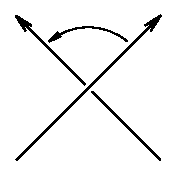
\includegraphics{images/crossing-right.pdf}
&
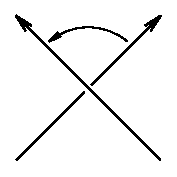
\includegraphics{images/crossing-left.pdf}
\\
+ & -
\end{tabular}

Хорды диаграммы Гаусса снабжены стрелками, ведущими по положительному направлению пересечения, и имеют подписи со знаками круток

\begin{tabular}{
>{\centering\arraybackslash}m{3cm}
>{\centering\arraybackslash}m{3cm}
}
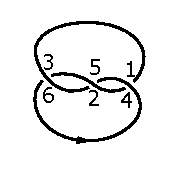
\includegraphics{images/sample-simple-knot.pdf}
&
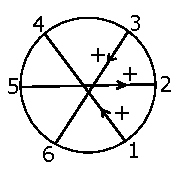
\includegraphics{images/sample-simple-knot-gauss.pdf}
\end{tabular}
